\documentclass[12pt, titlepage]{article}

\usepackage{booktabs}
\usepackage{tabularx}
\usepackage{hyperref}
\usepackage{fancyhdr}
\usepackage{float}
\usepackage{subcaption}
\usepackage{graphicx}

\pagestyle{fancy}
\hypersetup{
    colorlinks,
    citecolor=black,
    filecolor=blue,
    linkcolor=red,
    urlcolor=blue
}
\usepackage[round]{natbib}

% Test Counters
\newcounter{UInum}
\newcommand{\ttheUInum}{in-test-id \theUInum}
\newcommand{\UIref}[1]{in-test-id \ref{#1}}

\newcounter{LOGnum}
\newcommand{\ttheLOGnum}{log-test-id \theLOGnum}
\newcommand{\LOGref}[1]{log-test-id \ref{#1}}

\newcounter{GLnum}
\newcommand{\ttheGLnum}{logistic-test-id \theGLnum}
\newcommand{\GLref}[1]{logistic-test-id \ref{#1}}

\newcounter{USnum}
\newcommand{\ttheUSnum}{survey-ques-id \theUSnum}
\newcommand{\USref}[1]{survey-ques-id \ref{#1}}

\title{SE 3XA3: Test Report\\Ultimate Tic Tac Toe}

\author{Team 3,
		\\ Kunal Shah - shahk24
		\\ Pareek Ravi - ravip2
}

\date{\today}

%% Comments

\usepackage{color}

\newif\ifcomments\commentstrue

\ifcomments
\newcommand{\authornote}[3]{\textcolor{#1}{[#3 ---#2]}}
\newcommand{\todo}[1]{\textcolor{red}{[TODO: #1]}}
\else
\newcommand{\authornote}[3]{}
\newcommand{\todo}[1]{}
\fi

\newcommand{\wss}[1]{\authornote{blue}{SS}{#1}}
\newcommand{\ds}[1]{\authornote{red}{DS}{#1}}
\newcommand{\mj}[1]{\authornote{red}{MSN}{#1}}
\newcommand{\mh}[1]{\authornote{red}{MH}{#1}}
\newcommand{\cm}[1]{\authornote{red}{CM}{#1}}


% team members should be added for each team, like the following
% all comments left by the TAs or the instructor should be addressed
% by a corresponding comment from the Team

\newcommand{\tm}[1]{\authornote{magenta}{Team}{#1}}


\begin{document}

\lhead{Team 3 - Test Report}
\rhead{Ultimate Tic Tac Toe}

\maketitle

\pagenumbering{roman}
\tableofcontents
\listoftables
\listoffigures

\newpage
\begin{table}[hp]
\caption{\bf Revision History}
\begin{tabularx}{\textwidth}{p{3cm}p{2cm}X}
\toprule {\bf Date} & {\bf Version} & {\bf Notes}\\
\midrule
December 5 & 0.0 & Initial commit\\
December 6 & 0.1 & list of all tests\\
December 6 & 0.2 & Added figs to comparison section\\
December 7 & 0.3 & Fixed test counter\\
December 7 & 0.4 & Test trace to FR and MG\\

\bottomrule
\end{tabularx}
\end{table}

\newpage

\pagenumbering{arabic}

\section*{Abstract}
This document describes the results of all the testing done for Ultimate Tic Tac Toe.

\section{Functional Requirements Evaluation}
\subsection* {List of Functional Tests}

This section provides an overview of the functional tests completed. Tests are summarized in Table \ref{TbTestList}. 

\begin{table}[H]
\caption{\textbf{Table of Tests}} \label{TbTestList}
\begin{tabularx}{\textwidth}{p{3cm}X}
\toprule
\textbf{ID} & \textbf{Test} \\
\midrule

\UIref{UItest1} & Click should set random tile \\
\UIref{UItest2} & Win inner board \\
\UIref{UItest3} & Draw inner board (tie) \\
\LOGref{LOGtest1} & Win the full game\\
\LOGref{LOGtest2} & Draw the full game\\
\LOGref{LOGtest3} & Play Again\\
\LOGref{LOGtest4}  & Return to Board\\
\GLref{GLtest1} & Click on a cell that is already occupied \\
\GLref{GLtest2} & Users are alternating turns\\

\bottomrule
\end{tabularx}
\end{table}

\subsection{User Input}

\begin{itemize}

\item {\refstepcounter{UInum}\ttheUInum \label{UItest1}\\}
\textbf {Testing if user's input being received}
					
Initial State: It is the start of a new game and the board is empty
					
Input: A click on any random cell of any inner tic tac toe board
					
Expected Output: That cell should have the user's character on it

Actual Output: The cell contains that user's character

Result: The test passed
					
\item {\refstepcounter{UInum}\ttheUInum \label{UItest2}\\}
\textbf{Testing if user click on invalid inner board}
					
Initial State: Opponent has played on a inner board and it is the user's turn

Input: Click on a tile that they are not designated to click based on the
rules of the game
					
Expected Output: The board should not change at all. The game data should not change
and it is still the user's turn

Actual Output: Nothing happens

Result: The test passed

\item {\refstepcounter{UInum}\ttheUInum \label{UItest3}\\}
\textbf{Testing if user's input on cell already clicked}
					
Initial State: Opponent has played on a inner board and it is the user's turn
					
Input: Click on a tile that has already been clicked previously
					
Expected Output: The board should not change at all. The game data should not change
and it is still the user's turn

Actual Output: The cell doesn't change

Result: The test passed

\end{itemize}

\subsection{Game Logic}

\begin{itemize}

\item {\refstepcounter{LOGnum}\ttheLOGnum \label{LOGtest1}\\}
\textbf{Test if inner board gets completed}
					
Initial State: Inner board is almost completed by user. It is their turn to
play in the inner board where they will complete it.
					
Input: Clicks on the cell that will complete the inner board
					
Expected Output: The inner board will be marked with the character representing the
user

Actual Output: The inner board is marked with the character representing the player 
who completed the board

Result: The test passed

\item {\refstepcounter{LOGnum}\ttheLOGnum \label{LOGtest2}\\}
\textbf{Test if inner board ends in draw}
					
Initial State: The board is in a state where an inner board only has 1 cell
available to click and it will result in that board being a draw

Input: Click on the only available cell
					
Expected Output: The inner board will be marked with the character '-' meaning it is a
draw

Actual Output: The inner board is marked with '-'

Result: The test passed

\item {\refstepcounter{LOGnum}\ttheLOGnum \label{LOGtest3}\\}
\textbf{Test if next move can be made on any incomplete inner board}
					
Initial State: Game board is partially filled with one inner board completed

Input: Click at a cell corresponding to a completed inner board
					
Expected Output: All incomplete inner boards active

Actual Output: All the incomplete inner boards changed to an active board color

Result: The test passed

\item {\refstepcounter{LOGnum}\ttheLOGnum \label{LOGtest4}\\}
\textbf{Test if user turns are alternating}
					
Initial State: Player with character O or X just made a move

Input: Click at any available cell
					
Expected Output: The character on the other cell is the opposite

Actual Output: The character was the opposite

Result: The test passed

\end{itemize}
%\newpage
\subsection{Game Logistics}

\begin{itemize}

\item {\refstepcounter{GLnum}\ttheGLnum \label{GLtest1}\\}
\textbf{Test if game launches}
					
Initial State: User is in the file explorer
					
Input: User launches the html file in browser
					
Expected Output: The game launches in all browsers and shows the welcome dropdown

Actual Output: The game launches to the welcome dropdown in the user's preferred browser

Result: The test passed. 

Note: though the game does not work in Firefox, it has no issues in launching

\item {\refstepcounter{GLnum}\ttheGLnum \label{GLtest2}\\}
\textbf{Test if user input shows in window}
					
Initial State: User has just opened game
					
Input: User clicks on any cell
					
Expected Output: Cell they clicked on should change appearance

Actual Output: The cell on the game board shows the user's character

Result: The test passed

\end{itemize}

\section{Nonfunctional Requirements Evaluation}
Nonfunctional Requirements were tested using two methods, manual testing during the 
development of the game, and usability survey~\citep{survey} after revision 0 demonstration. After receiving feedback from beta testers' usability survey, changes where made to the application accordingly. Refer to section~\ref{ChangesAfterTesting} for details.

\subsection* {List of Survey Questions}

This section provides an overview of the survey questions asked in the usability survey. Questions are summarized in Table \ref{TbQuestionsList}. 

\begin{table}[H]
\caption{\textbf{Table of Questions}} \label{TbQuestionsList}
\begin{tabularx}{\textwidth}{p{3.1cm}X}
\toprule
\textbf{ID} & \textbf{Question} \\
\midrule

\USref{USq1} & The rules were very easy to find \\
\USref{USq2} & The rules are easy to understand \\
\USref{USq3} & The color pallet is visually appealing \\
\USref{USq4} & The response time was satisfying.\\
\USref{USq5} & It is clear which player's turn it is. (X or O)?\\
\USref{USq6} & The game runs smoothly on your browser\\
\USref{USq7} & Were you offended by anything in the game?\\
\USref{USq8} & Did you encounter epileptic symptoms while playing the game?\\
\USref{USq9} & Did anything unexpected appear on the screen while playing?\\
\USref{USq10} & Did you have fun playing this game?\\
\USref{USq11} & Any Additional Comments?\\


\bottomrule
\end{tabularx}
\end{table}

\subsection{Usability}

\begin{itemize}

\item {\refstepcounter{USnum}\ttheUSnum \label{USq1}\\}
\item {\refstepcounter{USnum}\ttheUSnum \label{USq2}\\}
\item {\refstepcounter{USnum}\ttheUSnum \label{USq3}\\}
\item {\refstepcounter{USnum}\ttheUSnum \label{USq4}\\}
\item {\refstepcounter{USnum}\ttheUSnum \label{USq5}\\}
\item {\refstepcounter{USnum}\ttheUSnum \label{USq6}\\}
\item {\refstepcounter{USnum}\ttheUSnum \label{USq7}\\}
\item {\refstepcounter{USnum}\ttheUSnum \label{USq8}\\}
\item {\refstepcounter{USnum}\ttheUSnum \label{USq9}\\}
\item {\refstepcounter{USnum}\ttheUSnum \label{USq10}\\}
\item {\refstepcounter{USnum}\ttheUSnum \label{USq11}\\}

\end{itemize}
		
\subsection{Performance}

	
\section{Comparison to Existing Implementation}
This project is a reimplementation of the original Ultimate tic tac toe game ~\citep{githubREF}. Prior to starting this project we investigated the existing implementation. There were 3 main elements we wanted to change for our reimplementation of Ultimate Tic Tac Toe which can been seen in Figure~\ref{fig:Comparison}.
\begin{enumerate}
\item Rules explaining how to play the game
\item User interface (colours and ascetic)
\item Ability to repay the game
\end{enumerate}

\begin{figure}[H]
\begin{subfigure}{.5\textwidth}
  \centering
  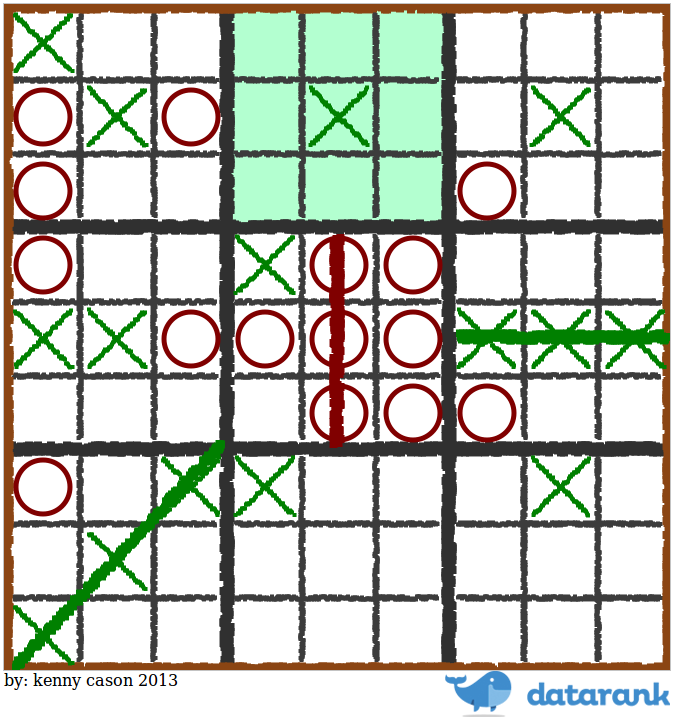
\includegraphics[width=0.95\linewidth]{../../ReferenceMaterial/SourceGame_screenshot.png}
  \caption{Original Game}
  \label{fig:sub1}
\end{subfigure}
\begin{subfigure}{.5\textwidth}
  \centering
  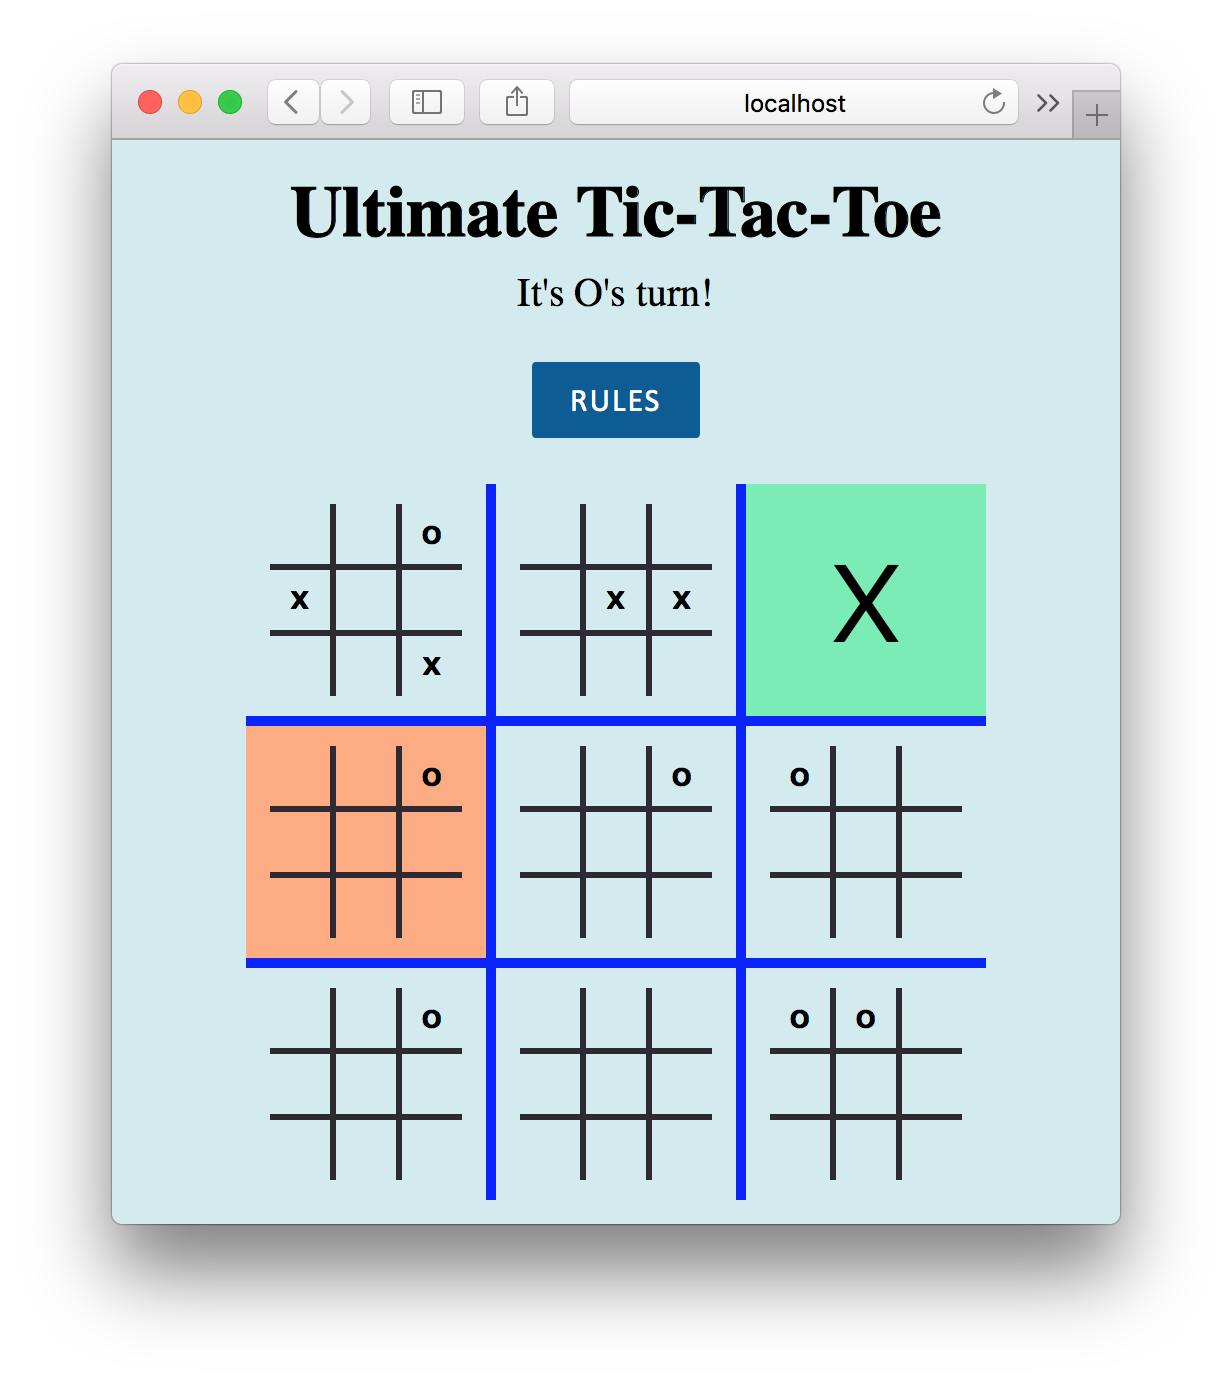
\includegraphics[width=1\linewidth]{../../ReferenceMaterial/XwinInnerBoard_screenshot.png}
  \caption{Reimplemented Game}
  \label{fig:sub2}
\end{subfigure}
\caption{Implementation Comparison}
\label{fig:Comparison}
\end{figure}

\section{Unit Testing}
\subsection{How to Test}
Unit testing was done using Karma and Jasmine frameworks. There is a folder called test
located in the src directory which contains the JavaScript file. In order to execute the testing framework, 
npm is required and all required packages are in a json file. Once all packages are installed, 
executing 'npm test' will run all the tests that are written in the test.js file.
\subsection{Tests}
The unit testing was done on the game logic which includes testing click functionality and some additional functionality such as the dropdown menus.
\section{Changes Due to Testing} \label{ChangesAfterTesting}
After performing unit testing on multiple browsers i.e.(Google Chrome, Safari, Firefox, Opera),
it was apparent that the game would not work on Firefox. The surveys also indicated that the game did
not work in Firefox. This was the only browser that was having issues with this. Unfortunately,
the reason for the incompatibility with Firefox is due to a click listener thus it could not be fixed. From
surveys, it was made clear that there was a scaling issue when playing on smaller displays, as such
changes were made to accommodate smaller devices screen sizes. The game board would adjust 
accordingly to the size of the display. The most common suggestion was to make it clear to 
\section{Automated Testing}
The automated testing was implemented with the Karma framework. This involved forcing Karma
to various game states and verifying if the results matched what was expected. The various 
states were a game ending in a win and ending in a draw.

\section{Trace to Requirements}
This section shows two traceability matrices: between the tests performed and the functional and non-functional requirements in \href{run:../SRS/SRS.pdf}{SRS}

\begin{table}[H]
\caption{\textbf{Trace to Functional Requirements}} \label{TbTrace}
\begin{tabularx}{\textwidth}{p{3cm}X}
\toprule
\textbf{Test ID} & \textbf{Functional Requirements ID} \\
\midrule

\UIref{UItest1} & FR1 , FR2,  \\
\UIref{UItest2} & FR3 \\
\UIref{UItest3} & FR4 \\
\LOGref{LOGtest1} & FR5\\
\LOGref{LOGtest2} & FR5\\
\LOGref{LOGtest3} & FR1\\
\LOGref{LOGtest4}  & FR1\\
\GLref{GLtest1} & FR2, FR6\\
\GLref{GLtest2} & FR6\\

\bottomrule
\end{tabularx}
\end{table}

\begin{table}[H]
\caption{\textbf{Trace to Non-Functional Requirements}} \label{TbTrace}
\begin{tabularx}{\textwidth}{p{3.1cm}X}
\toprule
\textbf{Test ID} & \textbf{Non-Functional Requirements ID} \\
\midrule

\USref{USq1} & FR1 , FR2,  \\
\USref{USq2} & FR3 \\
\USref{USq3} & FR4 \\
\USref{USq4} & FR5\\
\USref{USq5} & FR5\\
\USref{USq6} & FR1\\
\USref{USq7} & FR1\\
\USref{USq8} & FR2, FR6\\
\USref{USq9} & FR6\\
\USref{USq10} & FR6\\
\USref{USq11} & FR6\\

\bottomrule
\end{tabularx}
\end{table}
		
\section{Trace to Modules}		

\section{Code Coverage Metrics}

\bibliographystyle{plainnat}

\bibliography{TestReport}

\end{document}